\documentclass[12pt]{article}

\usepackage{scicite,times,graphicx,float,hyperref}
\usepackage[skip=0pt]{caption}
\usepackage[utf8]{inputenc}
\usepackage{enumitem}
\usepackage{booktabs}

\topmargin -1.0cm
\oddsidemargin 0.0cm
\textwidth 16cm 
\textheight 23cm
\footskip 1.0cm

\newenvironment{sciabstract}{%
\begin{quote} \bf}
{\end{quote}}

\newcounter{lastnote}
\newenvironment{scilastnote}{%
  \setcounter{lastnote}{\value{enumiv}}%
  \addtocounter{lastnote}{+1}%
  \begin{list}%
  {\arabic{lastnote}.}
  {\setlength{\leftmargin}{.22in}}
  {\setlength{\labelsep}{.5em}}
}
{\end{list}}

\title{Lab Work 3} 

\author
{André Pedrosa [85098], Filipe Pires [85122], João Alegria [85048]\\
\\
Algorithmic Information Theory\\
\normalsize{Department of Electronics, Telecommunications and Informatics}\\
\normalsize{University of Aveiro}\\
} 

\date{\today{}}

%%%%%%%%%%%%%%%%% END OF PREAMBLE %%%%%%%%%%%%%%%%

\begin{document} 

\baselineskip18pt

\maketitle 

\section{Introduction} %%%%%%%%%%%%%%%%%%%%%%%%%%%%%%%%%%%%%%%%%%%%%%%%%%%%%%%%%%%%%%%%%%%%%%%%%%%%%%%%%%%%%%%%%%%%%%%%%%%%%%%%%%%%%%%%%%%%%%%%%%%%%%%%%%%%%%%%%

This report aims to describe the work developed for the third and final assignment of the course of 'Algorithmic Information Theory', explaining all scripts
developed by us and presenting the results we considered most relevant regarding the quality of the solutions. 

The programs implemented in Shell have the purpose of measuring similarity of images using a compression-based strategy and automatically identify human faces.
Along with the description of the solutions, we also discuss the characteristics and the preprocessing done to the available dataset, the data compression 
algorithms used and the tests executed.
All code developed is publicly accessible in our GitHub repository: 

\url{https://github.com/joao-alegria/TAI}.
\newpage

\section{Image Classification} \label{classification} %%%%%%%%%%%%%%%%%%%%%%%%%%%%%%%%%%%%%%%%%%%%%%%%%%%%%%%%%%%%%%%%%%%%%%%%%%%%%%%%%%%%%%%%%%%%%%%%%%%%%%%%%%

When dealing with image processing problems that require object identification, the usual environment calls for a classification approach, as the objects to 
be identified belong to specific classes with clear and separable characteristics.
The challenge we are faced with \cite{trab3} is a special approach for the image classification problem of facial recognition or identification.
It is special in the sense that it does not aim to explore the usual strategies based on feature extraction, rather it is meant to rely on data compression 
methods and the notion of algorithmic information.
Algorithmic information, also known as algorithmic entropy or Kolmogorov complexity, is the measure of information in a given data portion based on the 
theoretical algorithm that would be required to recreate that same data portion. 

As this is an abstract definition, an example can clarify the concept: 
considering strings A="0101010101" and B="0010100110", for instance, one can easily reach the conclusion that string A is far easier to define than string B,
since for A we can simply define it as the smaller string "01" repeated 5 times; string B, on the other hand, the process is not as simple and we probably will
require the entire string to describe it.
What this means is that A has less information than B. 
To achieve the so called algorithmic information of each one, the thought process is the same but now the string descriptions are achieved through algorithms;
for our examples, the algorithms that define strings A and B are the following: 

\vspace{0.2in}
\begin{minipage}{0.45\textwidth}
  \begin{verbatim}
    def stringA():
      for i in range(5):
        print("01", end="")
  \end{verbatim}
\end{minipage}
\begin{minipage}{0.45\textwidth}
  \begin{verbatim}
    def stringB():
      for letter in "0010100110":
        print(letter, end="")
  \end{verbatim}
\end{minipage}
\vspace{0.2in}

By a quick analysis, it is obvious that \textit{stringA()} is less complex than \textit{stringB()}, iterating only 5 times, contrasting with the 10 iterations 
of the second; hence confirming that string B has more information than string A. 
This can be directly correlated with data compression, since compressors take advantage of the data repetition to reduce space usage, and thereby compress the 
information by storing the data that appears frequently and the indicators of the places where those repetitions occur.

With this in mind, one can proceed to understand how the image classification will be done. 
Using the Normalized Information Distance defined by equation \ref{eq:1}, where \textit{K(x)} and \textit{K(x|y)} define the Kolmogorov complexity of the 
string $x$ and of the string $x$ given string $y$. 

\begin{equation} \label{eq:1}
  NID(x,y) = \frac{max\{K(x|y),K(y|x)\}}{max\{K(x),K(y)\}}
\end{equation}
\newpage

Unfortunately, because the Kolmogorov complexity is non-computable, this formula is only theoretical and we are sure there is no algorithm that can compute 
any string complexity. 
Nevertheless, compressors approximate the formula's results very closely, if used correctly. 
So we used two of the most frequently used approximations of \texttt{NID} to determine the compression distance between images and, with these distances, 
calculate the closest images, i.e. the most similar ones, and hopefully classify them as belonging to the group of images that represent the same face.

\subsection{NCD Approximation} %%%%%%%%%%%%%%%%%%%%%%%%%%%%%%%%%%%%%%%%%%%%%%%%%%%%%%%%%%%

By using known general purpose compressors, such as gzip, lzma or tar, the Kolmogorov complexity can be estimated by the number of bits the resulting 
compressed file has. 
This approximation is called Normalized Compression Distance (NCD) and is expressed by equation \ref{eq:2}, where \textit{C(x)} and \textit{C(x,y)} represent 
the number of bits the compression of $x$ and of $x$ and $y$ concatenated contain, respectively.
The $xy$ concatenation can be performed in several ways, the most common being to simply perform an union on both; other more complex operations can also be done, 
such as interlacing the two data sources. 

\begin{equation}\label{eq:2}
  NCD(x,y) = \frac{C(x,y)-min\{C(x), C(y)\}}{max\{C(x),C(y)\}}
\end{equation}

Following the formula, results close to 0 indicate similarity and close to 1 dissimilarity. 
The only restriction to this approach is that the compressor used must follow the condition $C(x,x) \simeq C(x)$.
If this is not verified, the results of NCD are not reliable. 

\subsection{NCCD Approximation} %%%%%%%%%%%%%%%%%%%%%%%%%%%%%%%%%%%%%%%%%%%%%%%%%%%%%%%%%%

The second approximation is called Normalized Conditional Compression Distance, expressed by equation \ref{eq:3}.
The difference between NCD and NCCD is that the later uses conditional compressors to achieve its estimations. 
Conditional compressors are normally implemented with finite-context models and take in consideration the previous occurring terms to compress the new term. 
This is a more direct approximation of the NID and, in general, generates better results than the NCD.

\begin{equation}\label{eq:3}
  NCCD(x,y) = \frac{max\{C(x|y), C(y|x)\}}{max\{C(x), C(y)\}}
\end{equation}

\textit{C(x)} has the same meaning as before and \textit{C(x|y)} represents the number of bits the compression of $x$ needs given that $y$ occurred 
($C(y|x)$ follows the same logic). 
Due to the conditional aspect of this approach, \textit{C(x)} can be a special case of \textit{C(x|y)} were $y$ is equal to the empty string, making true the
statement $C(x) = C(x|\epsilon)$.

\newpage
\section{Dataset} %%%%%%%%%%%%%%%%%%%%%%%%%%%%%%%%%%%%%%%%%%%%%%%%%%%%%%%%%%%%%%%%%%%%%%%%%%%%%%%%%%%%%%%%%%%%%%%%%%%%%%%%%%%%%%%%%%%%%%%%%%%%%%%%%%%%%%%%%%%%%%

Like in all experimental work, specially in image processing, a considerably large dataset is required for any results to be significant and any conclusions to be solid.
Also, when benchmarking an algorithm, it is recommended that standard test datasets are used for researchers to be able to directly compare the results. 
Taking this in consideration, we downloaded AT\&T "The Database of Faces" (formerly "The ORL Database of Faces") and used it to test our code.

The image database contains 10 different images of each of the 40 distinct subjects.
For some subjects the images were taken at different times, between April 1992 and April 1994, with varying lighting conditions and different facial expressions.
Most faces are in an upright position in frontal view, with a slight left-right rotation.
All 400 images were taken in black \& white at the Olivetti Research Laboratory in Cambridge, UK.

\begin{figure}[H]
  \centering
  \begin{minipage}{\textwidth}
    \centering
    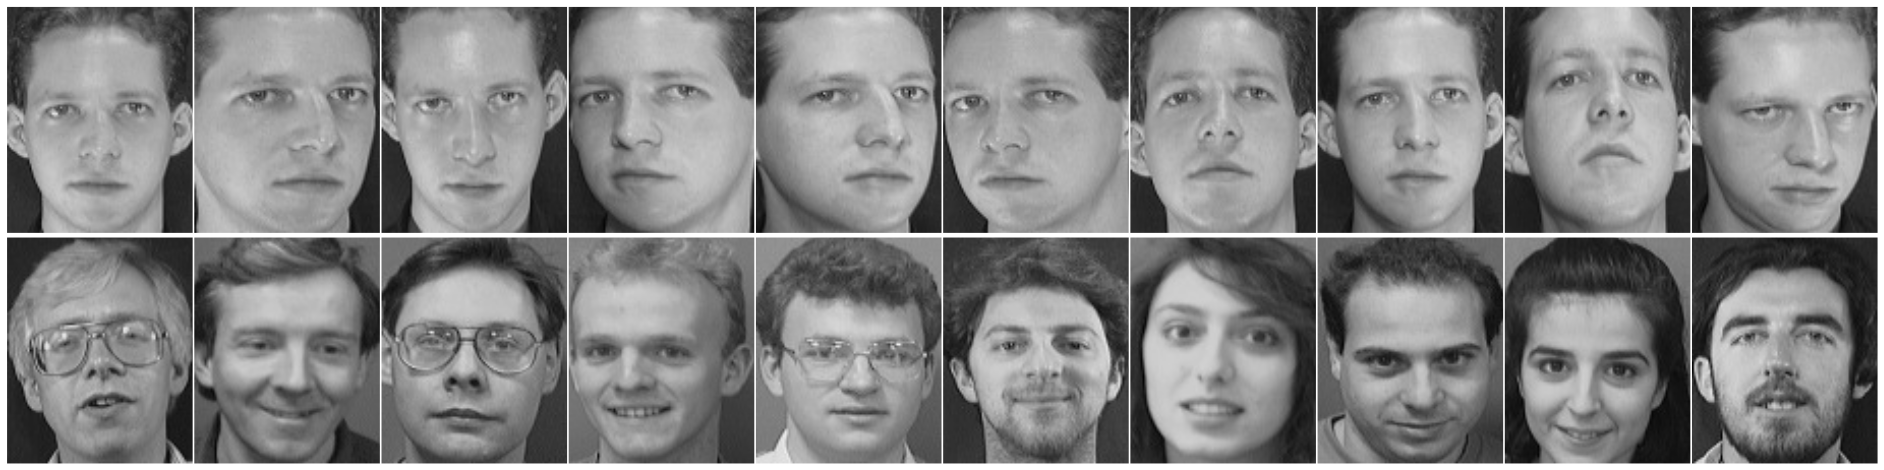
\includegraphics[width=\linewidth]{faces_example.png}
  \end{minipage}%
  \caption{Image taken from the assignment description \cite{trab3}. Examples from the ORL face dataset. In the first row, ten face images corresponding to the same subject (s01). In the second row, the first face image of subjects s02 to s11.}
  \label{fig:1}
\end{figure}

To speedup the processing of each image, we applied 2 transformations to each element of the dataset.
The first consisted in a simple image reduction from 112 $\times$ 92 px to 56 $\times$ 46 px, ensuring that proportions remained the same.
The second was a quantization process from 8 bits per pixel gray level to 4 bits only.
These modifications were accomplished using ImageMagick \cite{imgmagick}, a command-line program to create, edit, compose, or convert bitmap images.
The script developed to apply the transformations was \texttt{preprocessImages.sh}.

\begin{figure}[H]
  \centering
  \begin{minipage}{.2\textwidth}
    \centering
    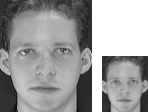
\includegraphics[width=\linewidth]{preprocessing_example.png}
  \end{minipage}%
  \caption{Example from subject s01 of the ORL face dataset, before and after preprocessing.}
  \label{fig:2}
\end{figure}

\newpage
\section{Experiment} %%%%%%%%%%%%%%%%%%%%%%%%%%%%%%%%%%%%%%%%%%%%%%%%%%%%%%%%%%%%%%%%%%%%%%%%%%%%%%%%%%%%%%%%%%%%%%%%%%%%%%%%%%%%%%%%%%%%%%%%%%%%%%%%%%%%%%%%%%%

Once the dataset was ready, we composed an experiment to determine which commonly used compressors provided the best results for our intents.
The conducted study had 2 phases: the first where we tested several data compressors using NCD and compared the precisions of the face identification 
program using each of the compressors; the second where we tested a conditional compressor using NCCD and compared the best results of the first phase with 
those of this test.

\subsection{Compressor Validation} \label{validation} %%%%%%%%%%%%%%%%%%%%%%%%%%%%%%%%%%%%

Before conducting our experiment, we needed to make sure the compressor candidates were valid.
This was done by verifying for each compressor \textit{C} if condition $C(x,x) \simeq C(x)$ was true.
The concatenation used in this verification uses the only valid operation for this situation, the "append" operation, which is explained in section \ref{pipeline}.

The script \texttt{checkCompressor.sh} was a script developed to help us manually verifying each compressor.
For each candidate, we compressed an example image and the concatenation of itself, and then ran this script.
What it does is collect the outcomes of the compressions and print them to the console side by side for us to quickly detect which break the condition.

From the compressors put to test, the ones we considered invalid were \texttt{pax} and \texttt{shar}, with a difference between \textit{C(x)} and \textit{C(x,x)}
of over 50\% for an example image as $x$, while the others were less than 40\%.
Although 40\% is still a very significant difference, we decided to keep most of the standard compressors as reaching a difference close to 0\% was already
known to be really difficult to find.

\subsection{Tested Compressors} %%%%%%%%%%%%%%%%%%%%%%%%%%%%%%%%%%%%%%%%%%%%%%%%%%%%%%%%%%

In this section we offer a small description of each of the validated standard compressors used in our experiment, chosen for their popularity and/or potential for our intentions.

Starting with \textbf{\texttt{zip}}, this command is a compression and file packaging utility for many OS, like Unix, VMS and MSDOS. 
It is analogous to a combination of the Unix commands \texttt{tar} and \texttt{compress} and it performs a lossless compression that can achieve 3:1/2:1 ratios. 
The standard compression method is \texttt{deflate}, which uses a combination of LZSS and Huffman coding.

Next we have \textbf{\texttt{gzip}}, a single-file/stream lossless data compression utility. 
This compression algorithm uses Lempel-Ziv coding (LZ77) to achieve its reduction factors. 
Gzip will only attempt to compress regular files and it will ignore symbolic links. 
Typically, text such as source code or English can be reduced by 60-70\%. 
Compression is generally much better than that achieved by LZW, Huffman coding, or adaptive Huffman coding.

\textbf{\texttt{bzip2}} is a free and open-source file compression program that uses the Burrows–Wheeler algorithm. 
It only compresses single files and is not a file archiver. 
This algorithm compresses most files more effectively than the older LZW and Deflate compression algorithms, but is considerably slower. 

The Lempel–Ziv–Markov chain algorithm, aslo known as \textbf{\texttt{lzma}}, is another algorithm used to perform lossless data compression. 
Developed by Igor Pavlov, it was first used in the 7z format of the 7-Zip archiver. 
This algorithm uses a dictionary compression scheme somewhat similar to the LZ77 algorithm.
It features a high compression ratio, generally higher than \texttt{bzip2} but less space-efficient.

\textbf{\texttt{zpaq}} is an open source command line archiver for Windows and Linux. 
It uses an append-only format which can be rolled back to an earlier state to retrieve older versions. 
It supports fast incremental update by adding only files whose last-modified date has changed since the previous update. 
It compresses using deduplication and several algorithms (LZ77, BWT, and context mixing) depending on the data type and the selected compression level.

Finally we have \textbf{\texttt{ppmd}}, Prediction by Partial Matching, an adaptive statistical data compression technique based on context modeling and prediction. 
PPM models use a set of previous symbols in the uncompressed symbol stream to predict the next symbol in the stream. 
PPM algorithms can also be used to cluster data into predicted groupings in cluster analysis.
\newline

The conditional compressor used to test NCCD was given \textit{a priori} for this assignment.
It is based on finite context modeling and it is implemented in C++ and specialized to compress images with the help of OpenCV.

\subsection{Study Pipeline} \label{pipeline} %%%%%%%%%%%%%%%%%%%%%%%%%%%%%%%%%%%%%%%%%%%%%

The experiment's pipeline is structured as an iterative process, built in \texttt{testCompressor.sh}.
This script receives as its only parameter the operation to be used to concatenate images.
As the concatenation can be done in more than one way, we executed the experiment for 3 different types of concatenations:
\vspace{-10pt}
\begin{itemize}[noitemsep]
  \item Append - this operation unites the two images one above the other (duplicating the height of the resulting image).
  \item Interlace - interpolated horizontal stripes of both images are stacked together (in this operation half of the data of each image is not used).
  \item Average - for each pixel position, the average of the gray value of both images at that position is calculated and added to the new image in the same position.
\end{itemize}
\vspace{-10pt}

\newpage
These image manipulations were also done with the help of ImageMagick and are defined for ease of access in \texttt{mergers.sh}.
Examples of these operations can be seen in Figure \ref{fig:3}, where the first 2 faces correspond to the first images of subjects s01 and s02, and the 
3 remaining images correspond to the concatenation using append, interlace and average respectively.
Note that, to verify the condition discussed in section \ref{validation}, the concatenation is done for the same image, so using either the average or the 
interlace operations will result in the exact same image as the original; this is why we used the append operation in that context.

\begin{figure}[H]
  \centering
  \begin{minipage}{.8\textwidth}
    \centering
    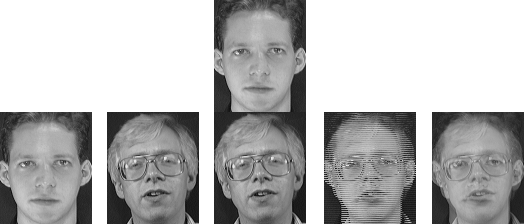
\includegraphics[width=\linewidth]{operations_example.png}
  \end{minipage}%
  \caption{Concatenation examples applied to subjects s01 and s02 using different operations.}
  \label{fig:3}
\end{figure}

Back to the experiment's script, its execution workflow follows the pseudo-code presented next, where \texttt{concat} corresponds to the chosen operation passed 
to the script and \texttt{compress} corresponds to the compression action executed by the current compressor of the first loop, defined in \texttt{compressors.sh}.

\begin{verbatim}
  for each compressor, do:
    for each subject, do:
      minNCD = 1
      for each testImg, do:
        for each goldStdImg, do:
          tmp = concat(testImg,goldStdImg)
          cTmp = compress(tmp)
          cT = compress(testImg)
          cGS = compress(goldStdImg)
          maxS = getMaxSize(cTmp,cT,cGS)
          minS = getMinSize(cTmp,cT,cGS)
          NCD = (size(cTmp) - minS) / maxS
          if NCD < minNCD:
            minNCD = NCD
\end{verbatim}

\newpage
The output of each script execution was written to disk in different files.
Then, to determine the performance of each compressor using each of the concatenation alternatives, we developed and executed a second script 
\texttt{calculateAccuracy.sh} that reads the output files, computes the accuracies and writes them on the console for analysis. 

Along with the instructions for this assignment and the programs already developed, an additional script was provided to us to test NCCD, \texttt{TEST123}.
To determine the performance of this solution, we developed \texttt{nccdAccuracy.sh} that does the same as \texttt{calculateAccuracy.sh} but for NCCD's output.

\section{Results \& Discussion} %%%%%%%%%%%%%%%%%%%%%%%%%%%%%%%%%%%%%%%%%%%%%%%%%%%%%%%%%%%%%%%%%%%%%%%%%%%%%%%%%%%%%%%%%%%%%%%%%%%%%%%%%%%%%%%%%%%%%%%%%%%%%%%%

The results of the first phase were quite promising, with some compressors achieving accuracy percentages of over 70\%.
Table \ref{tab:1} presents the performance of NCD using each compressor and each of the concatenation techniques.

\begin{table}[h!]
\centering
\begin{tabular}{@{}c|cccccc@{}}
                   & \textbf{\texttt{zip}} & \textbf{\texttt{gzip}} & \textbf{\texttt{lzma}} & \textbf{\texttt{bzip2}} & \textbf{\texttt{zpaq}} & \textbf{\texttt{ppmd}}\\ \midrule
\textbf{Append}    & 0.707     & \textbf{0.725}   & 0.271           & 0.507     & 0.060           & 0.657 \\
\textbf{Interlace} & 0.100     & 0.560            & \textbf{0.682}  & 0.578     & 0.021           & 0.025 \\ 
\textbf{Average}   & 0.021     & 0.021            & 0.014           & 0.042     & \textbf{0.089}  & 0.025 \\ 
\end{tabular}
\vspace{5pt}
\caption{Accuracy for each compressor using different concatenation operations.}
\label{tab:1}
\end{table}

The best compressor using the concatenation type "append" was \texttt{gzip}, using "interlace" was \texttt{lzma} and using "average" was \texttt{zpaq}.
However, the average operation presented extremely low accuracies, failing to classify the faces over 90\% of the time.
Our understanding is that, ...........................
% explain why average is so bad

Now, the reason why append presents better results than interlace is that ....................
% explain why append is better

But these results are very much dependent on the compression algorithms used, as one can see by the difference of accuracies amongst compressors using the same operation.
The fact that \texttt{lzma} ............... might have been very much beneficial when faced with an interlace-type concatenation.
The inverse seems to have happened to \texttt{zip}, possibly because ..................
% explain the big difference of accuracy between concatenation types for zip and lzma

Because "append" presented the highest performance on almost all compressors, we decided to discard the other two operators for the remaining of the experiment.
Because \texttt{gzip} showed the best accuracy and presented itself as the most robust standard compressor (taking in consideration that its accuracy was also
amongst the highest using "interlace"), we decided to proceed to the next phase with this compressor.
\newline 

To calculate the performance of NCCD, we executed \texttt{nccdAccuracy.sh} after running \texttt{TEST123} for all dataset images.
The accuracy of this solution was \textbf{0.617}, about 10\% worst than the best alternative of NCD.
Theoretically, NCCD should deliver better results than NCD, since the algorithm is a more direct approximation to NID, discussed in chapter \ref{classification},
and a conditional compressor would benefit very much from processing faces, as they have many visual patterns to be explored.
And this is verified when compared to NCD with most of the tested compressors.
But, although surprising, it is not too hard to believe that NCD with \texttt{gzip} compression surpassed NCCD when compared in terms of accuracy for face 
identification, as the difference is significant but not exaggerated.

\newpage
\section{Conclusions} %%%%%%%%%%%%%%%%%%%%%%%%%%%%%%%%%%%%%%%%%%%%%%%%%%%%%%%%%%%%%%%%%%%%%%%%%%%%%%%%%%%%%%%%%%%%%%%%%%%%%%%%%%%%%%%%%%%%%%%%%%%%%%%%%%%%%%%%%%

After completing the assignment, we drew a few conclusions regarding the topics here explored and our endeavor to deliver work of quality.

The first aspect worth mentioning is how refreshing was the idea of tackling a classification problem through an unconventional strategy.
The connection between the studied concepts and the project's goals were quite captivating.

The implementation was also interesting, since we decided to adopt Shell scripting and were able to work in close contact with the compression commands.
Exploring the characteristics and capabilities of compressors we use on an almost daily bases will be very useful for future tasks requiring compression algorithms.

Finally, the levels of accuracy that the solutions achieved were quite impressive to us.
Since we were used to developing machine learning approaches for problems relatively similar to this, we expected to see poor results from a solution that did 
not interpret the data in the conventional way.
We were very much satisfied with the final results and the delivered work, as it accomplishes all objectives of the assignment.

In terms of code organization and readability, we made sure our repository was as well structured as possible and our code properly commented.
The base folder contains a \textit{README} file for basic instructions.
The \textit{src} and \textit{examples} folders contain the code and other resources made available for the project (not developed by us), our scripts are on the base folder.
The dataset is present in \textit{orl\_faces}, and the preprocessed images in \textit{processedFaces}.
The folder \textit{experiments} contains the results of our studies and the scripts to calculate the performance of the solutions.

\begin{thebibliography}{9} %%%%%%%%%%%%%%%%%%%%%%%%%%%%%%%%%%%%%%%%%%%%%%%%%%%%%%%%%%%%%%%%%%%%%%%%%%%%%%%%%%%%%%%%%%%%%%%%%%%%%%%%%%%%%%%%%%%%%%%%%%%%%%%%%%%%%
  \bibliographystyle{Science}

  \bibitem{trab3}
    Armando J. Pinho,
    \textit{AIT: Lab Work no.3},
    University of Aveiro,
    2019/20.
  
  \bibitem{imgmagick}
    ImageMagick Studio LLC,
    \textit{ImageMagick},
    \url{https://imagemagick.org/index.php},
    accessed in December 2019.
  
\end{thebibliography}

\clearpage

\end{document}




















